%
% File: chap01.tex
% Author: Victor F. Brena-Medina
% Description: Introduction chapter where the biology goes.
%
\let\textcircled=\pgftextcircled
\chapter{The Peripheral Circuits}
\label{chap:peripherals}

\section{Overview}
\paragraph{}

In the previous chapter, we studied about the Logical and Arithmetic operations that have been included in our In-Memory Compute. In order to perform the select, read operations for the operands that have to be operated and write operation for writing back the computed value to the memory address, peripheral circuits are needed. In this section we will discuss the the Row decoder, Write driver and the Pre-Charge circuits. 

\section{Row Decoder}
\paragraph{}
A 2x4 Row Decoder with enable functionality is used to enable one of the row out of four rows in the 4x8 memory array. Each row of  the decoder consists of a two input NOR gate and two NOT gates, one of which has an active low enable that produces HIGH output of the row when pulled low. The 2 bit address is used to refer to the row that has to be selected. The method of Logical Effort was used in order to reduce the delay time of the path by appropriate sizing of gates.


\begin{figure}[H]
\centering
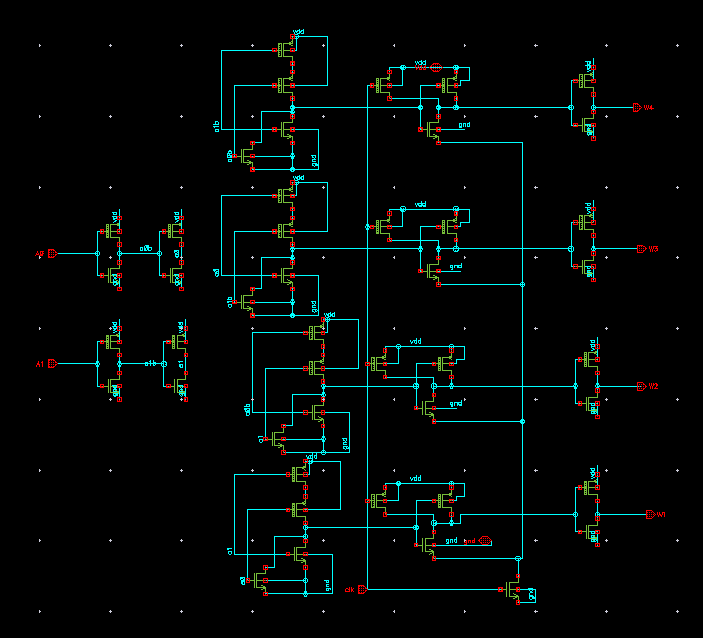
\includegraphics[width=0.7\textwidth]{row_decoder.png}
\caption{Row Decoder}
\label{fig:Figure}
\end{figure}

The expressions for the rows are:

\begin{itemize}
\item RL1 =  $\overline{( A1 +  A0)}$.(enable)
\item RL2 =  $\overline{( A1 + \overline{A0})}$.(enable) 
\item RL3 =  $\overline{(\overline{A1} +  A0)}$.(enable) 
\item RL4 =  $\overline{(\overline{A1} + \overline{A0})}$.(enable)
\end{itemize}

\section{Write Driver}
\paragraph{}

The write driver has the function of writing back the output of the computation into the desired cell. It also has the functionality of writing any other external data to the cell. One of the functionality can be selected through a MUX which is made up transmission gates. The write driver drives the WBL and WBLB rail to rail, ensuring proper writing into the 8T SRAM cell.

\begin{figure}[H]
\centering
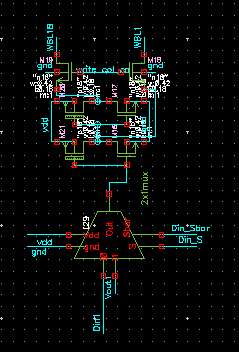
\includegraphics[width=0.5\textwidth]{write_driver.png}
\caption{Write Driver}
\label{fig:Figure}
\end{figure}


\section{Write and Read Pre-Charge}
\paragraph{}

The Write and Read Precharge are used just before writing or reading into the SRAM to pull-up the bit lines.  


\begin{figure}[H]
\centering
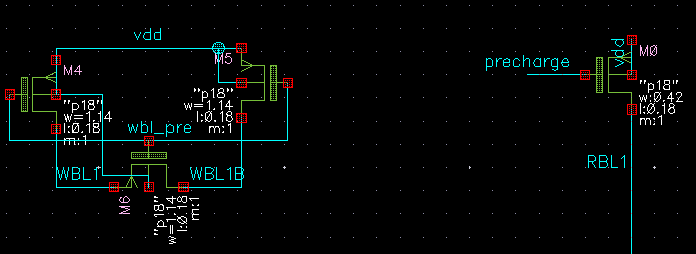
\includegraphics[width=0.7\textwidth]{write_read_precharge.png}
\caption{Write and Read Pre-Charge}
\label{fig:Figure}
\end{figure}

